% figures/loan-state-machine.tex
\documentclass[11pt]{article}
\usepackage[margin=1.5cm]{geometry}
\usepackage{tikz}
\usetikzlibrary{positioning,arrows.meta}
\pagestyle{empty}
\begin{document}
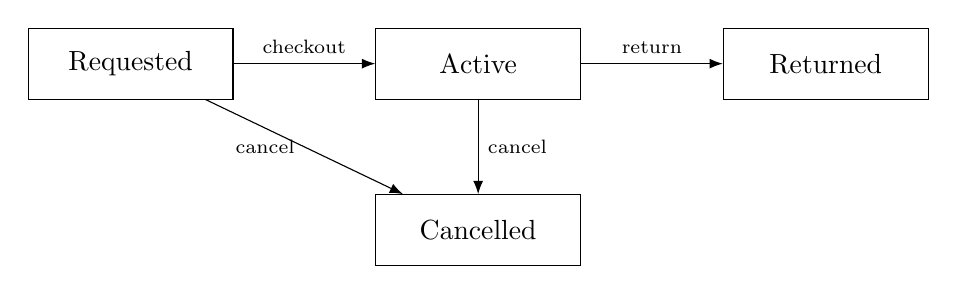
\begin{tikzpicture}[node distance=18mm, >=Latex]
  \node[draw, rectangle, minimum width=2.6cm, minimum height=0.9cm] (requested) {Requested};
  \node[draw, rectangle, minimum width=2.6cm, minimum height=0.9cm, right=18mm of requested] (active) {Active};
  \node[draw, rectangle, minimum width=2.6cm, minimum height=0.9cm, right=18mm of active] (returned) {Returned};
  \node[draw, rectangle, minimum width=2.6cm, minimum height=0.9cm, below=12mm of active] (cancelled) {Cancelled};

  \draw[->] (requested) -- (active) node[midway, above, font=\scriptsize] {checkout};
  \draw[->] (active) -- (returned) node[midway, above, font=\scriptsize] {return};
  \draw[->] (requested) -- (cancelled) node[midway, left, font=\scriptsize] {cancel};
  \draw[->] (active) -- (cancelled) node[midway, right, font=\scriptsize] {cancel};
\end{tikzpicture}
\end{document}
